\subsection{Test di Validazione}
I test di validazione saranno identificati secondo quanto riportato nel documento \NPdoc{}.
\normalsize
\begin{longtable}{|c|>{}m{8cm}|c|}
\hline
\textbf{Id Test} & \textbf{Descrizione} & \textbf{Stato}\\
\hline
\endhead
\hypertarget{TVFO1}{TVFO1} & L'utente deve verificare che il sistema riesca a riconoscerlo come ospite o possibile amministratore. All'utente viene richiesto di:
\begin{itemize}
\item fornire nome e cognome;
\end{itemize} & \textit{Non Implementato}\\ \hline
\hypertarget{TVFO1.1.2}{TVFO1.1.2} & L'utente deve verificare che il sistema ne permetta l'accesso all'area amministrativa tramite l'assistente virtuale. All'utente viene richiesto di:
\begin{itemize}
\item comunicare i propri dati identificativi;
\item verificare che il sistema riconosca l'utente come un possibile amministratore non autenticato;
\item comunicare l'intento di volersi autenticare come amministratore;
\item comunicare la frase per lo Speaker Recognition;
\item verificare l'accesso all'area amministrativa.
\end{itemize} & \textit{Non Implementato}\\ \hline
\hypertarget{TVFO2.1}{TVFO2.1} & L'utente deve verificare che il sistema permetta la creazione di una nuova direttiva. All'utente viene richiesto di:
\begin{itemize}
\item autenticarsi come amministratore;
\item comunicare l'intento di voler creare una nuova direttiva;
\item inserire il nome della direttiva;
\item inserire la funzione della direttiva;
\item inserire il target della direttiva;
\item confermare la creazione della direttiva;
\item verificare che la direttiva sia stata creata correttamente.
\end{itemize}
 & \textit{Non Implementato}\\ \hline
\hypertarget{TVFO2.1.1.6}{TVFO2.1.1.6} & L'utente deve verificare che, durante la creazione di una direttiva, l'inserimento di dati non validi (funzione o target della direttiva inesistenti) comporti la visualizzazione di un messaggio d'errore. All'utente viene richiesto di:
\begin{itemize}
\item autenticarsi come amministratore;
\item comunicare l'intento di voler creare una nuova direttiva;
\item inserire il nome della direttiva;
\item inserire una funzione per la direttiva che non sia valida (inesistente);
\item inserire un target per la direttiva che non sia valido (inesistente);
\item verificare la comparsa di un messaggio d'errore.
\end{itemize} & \textit{Non Implementato}\\ \hline
\hypertarget{TVFO2.1.2}{TVFO2.1.2} & L'utente deve verificare che il sistema permetta l'eliminazione di una direttiva. All'utente viene richiesto di:
\begin{itemize}
\item autenticarsi come amministratore;
\item comunicare l'intento di voler eliminare una direttiva;
\item comunicare il nome della direttiva da eliminare;
\item confermare l'eliminazione della direttiva;
\item verificare che la direttiva sia stata eliminata correttamente.
\end{itemize}
 & \textit{Non Implementato}\\ \hline
\hypertarget{TVFO2.1.4}{TVFO2.1.4} & L'utente deve verificare che il sistema permetta la visualizzazione di una direttiva. All'utente viene richiesto di:
\begin{itemize}
\item autenticarsi come amministratore;
\item comunicare l'intento di voler visualizzare una direttiva;
\item verificare che il sistema permetta la visualizzazione di nome, funzione, target,funzionalità e abilitazione della direttiva.
\end{itemize} & \textit{Non Implementato}\\ \hline
\hypertarget{TVFO2.2}{TVFO2.2} & L'utente deve verificare che il sistema permetta la modifica dei dati del proprio profilo. All'utente viene richiesto di:
\begin{itemize}
\item autenticarsi come amministratore;
\item comunicare l'intento di voler modificare il proprio profilo;
\item comunicare nome e cognome;
\item confermare la modifica;
\item verificare che la modifica sia stata effettuata;
\end{itemize}
 & \textit{Non Implementato}\\ \hline
\hypertarget{TVFO3.1}{TVFO3.1} & L'utente deve verificare che sia possibile comunicare al sistema la persona che si desidera incontrare. All'utente viene richiesto di:
\begin{itemize}
\item aver comunicato i propri dati al sistema ed essere riconosciuti come ospiti;
\item comunicare la persona che si desidera raggiungere;
\item verificare che il sistema abbia capito le informazioni comunicate;
\end{itemize} & \textit{Non Implementato}\\ \hline
\hypertarget{TVFO5}{TVFO5} & L'utente deve verificare che, nel caso in cui il sistema nel caso non riesca ad interpretare la risposta, chieda nuovamente l'informazione all'utente. All'utente viene richiesto di:
\begin{itemize}
\item comunicare al sistema qualcosa che non può essere interpretato da esso;
\item verificare che il sistema richieda nuovamente l'informazione.
\end{itemize} & \textit{Non Implementato}\\ \hline
\hypertarget{TVFO7}{TVFO7} & L'utente deve verificare che, nel caso in cui esso sia già stato un ospite in passato, il sistema lo riconosca. All'utente viene richiesto di:
\begin{itemize}
\item aver comunicato i propri dati al sistema ed essere riconosciuti come ospiti;
\item verificare che il sistema riconosca l'utente come qualcuno che è già stato un ospite in passato.
\end{itemize}
 & \textit{Non Implementato}\\ \hline
\caption[Test di Validazione]{Test di Validazione}
\label{tabella:test0}
\end{longtable}
\clearpage

\subsection{Test di Sistema}
I test di sistema saranno identificati secondo quanto riportato nel documento \NPdoc{}.
\normalsize
\begin{longtable}{|c|>{}m{8cm}|c|}
\hline
\textbf{Id Test} & \textbf{Descrizione} & \textbf{Stato}\\
\hline
\endhead
\hypertarget{TSFO1}{TSFO1} & Il sistema deve poter riconoscere un utente come ospite. & \textit{Non Implementato}\\ \hline
\hypertarget{TSFO1.1.2.1}{TSFO1.1.2.1} & Il sistema deve permettere all'utente di autenticarsi come amministratore tramite frase di riconoscimento. & \textit{Non Implementato}\\ \hline
\hypertarget{TSFO2.1.1}{TSFO2.1.1} & Il sistema deve permettere all'amministratore di poter creare una nuova direttiva. & \textit{Non Implementato}\\ \hline
\hypertarget{TSFO2.1.2}{TSFO2.1.2} & Il sistema deve permettere all'amministratore di poter eliminare una direttiva di cui ha i privilegi. & \textit{Non Implementato}\\ \hline
\hypertarget{TSFO2.1.4}{TSFO2.1.4} & Il sistema deve permettere all'amministratore di poter visualizzare le direttive di cui ha i privilegi. & \textit{Non Implementato}\\ \hline
\hypertarget{TSFO2.2.1}{TSFO2.2.1} & L'amministratore deve poter modificare il nome e cognome del suo profilo. & \textit{Non Implementato}\\ \hline
\hypertarget{TSFO3.1}{TSFO3.1} & Il sistema deve permettere all'ospite di richiedere la persona desiderata. & \textit{Non Implementato}\\ \hline
\hypertarget{TSFO5}{TSFO5} & Il sistema deve richiedere nuovamente le informazioni nel caso in cui non fossero state comprese. & \textit{Non Implementato}\\ \hline
\hypertarget{TSFO7}{TSFO7} & Il sistema deve essere in grado di riconoscere ospiti già stati in visita all'azienda. In questo caso, l'assistente virtuale deve poter prevedere le sue necessità. & \textit{Non Implementato}\\ \hline
\hypertarget{TSFO8}{TSFO8} & Il sistema deve sollecitare la persona desiderata o eventualmente avvisare gli altri membri dell'azienda su richiesta dell'ospite. & \textit{Non Implementato}\\ \hline
\hypertarget{TSFO13}{TSFO13} & Il sistema deve comunicare nell'opportuno canale di Slack le informazioni raccolte durante l'interazione con l'ospite. & \textit{Non Implementato}\\ \hline
\hypertarget{TSVO1.1}{TSVO1.1} & Vogliamo testare che il software funzioni correttamente in un PC con sistema operativo Windows 7 o superiore.
 & \textit{Non Implementato}\\ \hline
\hypertarget{TSVO4}{TSVO4} & Le pagine HTML devono essere validate. & \textit{Non Implementato}\\ \hline
\hypertarget{TSVO5}{TSVO5} & I fogli di stile CSS devono essere validati. & \textit{Non Implementato}\\ \hline
\hypertarget{TSVO10}{TSVO10} & Vogliamo testare che il software funzioni correttamente con il browser Google Chrome versione 53 o superiore. & \textit{Non Implementato}\\ \hline
\caption[Test di Sistema]{Test di Sistema}
\label{tabella:test1}
\end{longtable}
\clearpage

\subsection{Test di Integrazione}
I test di integrazione saranno identificati secondo quanto riportato nel documento \NPdoc{}.\\
Segue il diagramma di attività relativo ai test d'integrazione.
\begin{figure}[h]
	\centering
	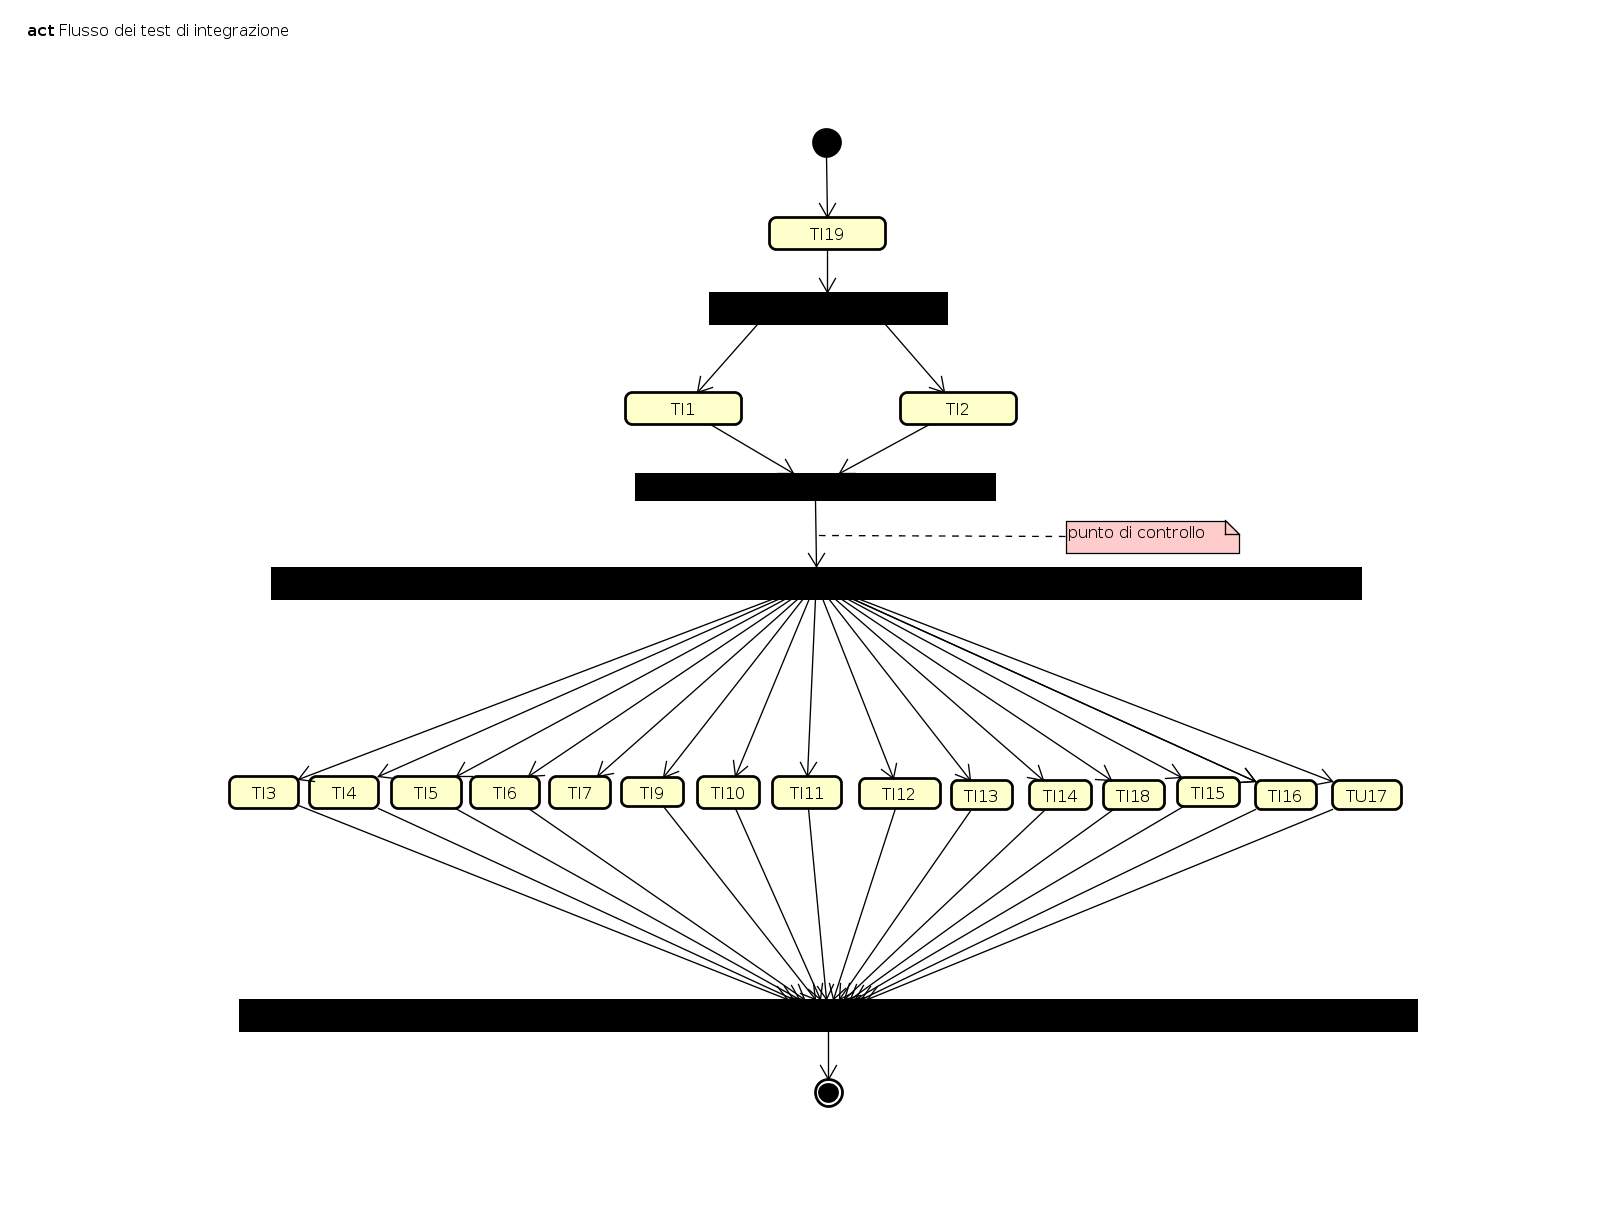
\includegraphics[width=\textwidth,height=\textheight,keepaspectratio]{FlussoIntegrazione.png}
	\caption{Diagramma di attività dei test d'integrazione}
\end{figure}
\normalsize
\begin{longtable}{|c|>{}m{8cm}|c|}
\hline
\textbf{Id Test} & \textbf{Descrizione} & \textbf{Stato}\\
\hline
\endhead
\hypertarget{TI1}{TI1} & Vogliamo verificare che \file{Recorder}, \file{Logic}, \file{Utility}, \file{Recorder}, \file{TTS}, \file{ConversationApp} e \file{ApplicationManager} interagiscano correttamente fra loro. & \textit{Non Implementato}\\ \hline
\hypertarget{TI2}{TI2} & Vogliamo verificare che \file{APIGateway}, \file{STT}, \file{VirtualAssistant},  \file{Users}, \file{Guests}, \file{Rules}, \file{Members}, \file{Conversations} e \file{Events} interagiscano correttamente tra di loro. Inoltre, vogliamo verificare che interagiscano correttamente con i servizi e librerie esterne AWS, Speaker Recognition, Speech to text IBM Watson, api.ai, Slack e \file{WebAPI}. & \textit{Non Implementato}\\ \hline
\hypertarget{TI3}{TI3} & Vogliamo verificare che le seguenti classi, contenute in \file{Client::ApplicationManager}, interagiscano tra loro correttamente: \file{ApplicationManagerObserver}, \file{ApplicationRegistryClient}, \file{ApplicationRegistryLocalClient}, \file{ApplicationLocalRegistry}, \file{Manager}, \file{State}, \file{Application}, \file{ApplicationPackage}. & \textit{Non Implementato}\\ \hline
\hypertarget{TI4}{TI4} & Vogliamo verificare che le seguenti classi, contenute in \file{Client::Logic}, interagiscano tra loro correttamente: \file{DataArrivedSubject}, \file{DataArrivedObservable}, \file{Logic}, \file{HttpError}, \file{HttpPromise}, \file{LogicObserver}. & \textit{Non Implementato}\\ \hline
\hypertarget{TI5}{TI5} & Vogliamo verificare che le seguenti classi, contenute in \file{Client::Recorder}, interagiscano tra loro correttamente: \file{Recorder}, \file{RecorderWorker}, \file{RecorderMsg}, \file{RecorderWorkerMsg}, \file{RecorderWorkerConfig}, \file{RecorderConfig}, \file{SpeechEndSubject}, \file{SpeechEndObservable}. & \textit{Non Implementato}\\ \hline
\hypertarget{TI6}{TI6} & Vogliamo verificare che le seguenti classi, contenute in \file{Client::TTS}, interagiscano tra loro correttamente: \file{TTSConfig}, \file{Player}, \file{PlayerObserver}. & \textit{Non Implementato}\\ \hline
\hypertarget{TI7}{TI7} & Vogliamo verificare che le seguenti classi, contenute in \file{Client::Utility}, interagiscano tra loro correttamente: \file{BoolSubject}, \file{BoolObservable}, \file{BoolObserver}. & \textit{Non Implementato}\\ \hline
\hypertarget{TI8}{TI8} & Vogliamo verificare che le seguenti classi, contenute in \file{Back-end::APIGateway}, interagiscano tra loro correttamente: \file{VocalAPI}, \file{Enrollement}. & \textit{Non Implementato}\\ \hline
\hypertarget{TI9}{TI9} & Vogliamo verificare che le seguenti classi, contenute in \file{Back-end::Users}, interagiscano tra loro correttamente: \file{UsersDAODynamoDB}, \file{User}, \file{UsersService}. & \textit{Non Implementato}\\ \hline
\hypertarget{TI10}{TI10} & Vogliamo verificare che le seguenti classi, contenute in \file{Back-end::Rules}, interagiscano tra loro correttamente: \file{Rule}, \file{RulesDAODynamoDB}, \file{RuleTarget}, \file{RuleTaskInstance}, \file{RulesService}, \file{TasksDAODynamoDB}, \file{Task}. & \textit{Non Implementato}\\ \hline
\hypertarget{TI11}{TI11} &
Vogliamo verificare che le seguenti classi, contenute in \file{Back-end::VirtualAssistant}, interagiscano tra loro correttamente: \file{VAService}, \file{ApiAIVAAdapter}, \file{VAQuery}, \file{Agent}, \file{AgentDAODynamoDB}, \file{VAEventObject}, \file{Fulfillment}, \file{MsgObject}, \file{ButtonObject}. & \textit{Non Implementato}\\ \hline
\hypertarget{TI12}{TI12} & Vogliamo verificare che le seguenti classi, contenute in \file{Back-end::Member}, interagiscano tra loro correttamente: \file{MembersSlackDAO}, \file{Member}. & \textit{Non Implementato}\\ \hline
\hypertarget{TI13}{TI13} & Vogliamo verificare che le seguenti classi, contenute in \file{Back-end::Guests}, interagiscano tra loro correttamente: \file{Guest}, \file{GuestDAODynamoDB}. & \textit{Non Implementato}\\ \hline
\hypertarget{TI14}{TI14} & Vogliamo verificare che le seguenti classi, contenute in \file{Back-end::Conversations}, interagiscano tra loro correttamente: \file{ConversationDAODynamoDB}, \file{Conversation}, \file{ConversationMsg}.
 & \textit{Non Implementato}\\ \hline
\hypertarget{TI15}{TI15} & Vogliamo verificare che le seguenti classi, contenute in \file{Back-end::Events}, interagiscano tra loro correttamente: \file{SNSRecord}, \file{SNSMessage}.
 & \textit{Non Implementato}\\ \hline
\hypertarget{TI16}{TI16} & Vogliamo verificare che le seguenti classi, contenute in \file{Back-end::Notifications}, interagiscano tra loro correttamente: \file{NotificationChannel}, \file{Purpose}, \file{Topic}, \file{NotificationMessage}, \file{Attachment}, \file{Action}, \file{ConfirmationFields}. & \textit{Non Implementato}\\ \hline
\hypertarget{TI17}{TI17} & Vogliamo verificare che le seguenti classi, contenute in \file{Back-end::Utility}, interagiscano tra loro correttamente: \file{WebhookRequest}, \file{ProcessingResult}, \file{LamdaIdEvent}, \file{PathIdParam}. & \textit{Non Implementato}\\ \hline
\hypertarget{TI18}{TI18} & Vogliamo verificare che le seguenti classi, contenute in \file{Client::ConversationApp}, interagiscano tra loro correttamente: \file{ConversationApp}, \file{ConversationActionObserver}, \file{ConversationActionObservable}, \file{ConversaionActionSubject}, \file{ConversationAction}, \file{ConversationDispatcher}, \file{ConversationView}, \file{MessageStore}. & \textit{Non Implementato}\\ \hline
\hypertarget{TI19}{TI19} & Vogliamo verificare che \file{Client} e \file{Back-end} interagiscano tra loro correttamente. & \textit{Non Implementato}\\ \hline
\caption[Test di Integrazione]{Test di Integrazione}
\label{tabella:test2}
\end{longtable}
\clearpage

\subsection{Test di Unità}
I test di unita saranno identificati secondo quanto riportato nel documento \NPdoc{}.
\normalsize
\begin{longtable}{|c|>{}m{8cm}|c|}
\hline
\textbf{Id Test} & \textbf{Descrizione} & \textbf{Stato}\\
\hline
\endhead
\hypertarget{TU1}{TU1} & Vogliamo testare che il metodo imposta il campo \file{status} della risposta a 200 e il campo \file{speech} sia uguale al campo \file{fulfillment.speech} del corpo della richiesta, in caso il token sia presente e valido. & \textit{Non Implementato}\\ \hline
\hypertarget{TU2}{TU2} & Vogliamo testare che il metodo imposta il campo \file{status} della risposta a 403 in caso di mancata autenticazione, ovvero token assente o non valido. & \textit{Non Implementato}\\ \hline
\hypertarget{TU3}{TU3} & Vogliamo testare che il metodo solleva un'eccezione alla sua chiamata. & \textit{Non Implementato}\\ \hline
\hypertarget{TU4}{TU4} & Vogliamo testare che il metodo accetta un parametro di tipo \file{Agent} senza generare eccezioni. & \textit{Non Implementato}\\ \hline
\hypertarget{TU5}{TU5} & Vogliamo testare che il metodo solleva un eccezione nel caso in cui il parametro non sia di tipo \file{Agent}. & \textit{Non Implementato}\\ \hline
\hypertarget{TU6}{TU6} & Vogliamo testare che se la chiamata al servizio di STT non va a buon fine, venga chiamato il metodo \file{succeed} del \file{context}, con un parametro \file{LambdaResponse} avente \file{statusCode} pari a 500. & \textit{Non Implementato}\\ \hline
\hypertarget{TU7}{TU7} & Vogliamo testare che se lo \file{status} della risposta ricevuta dall'assistente virtuale sia diverso da 200, venga chiamato il metodo \file{succeed} di \file{context} con un oggetto di tipo \file{LambdaResponse} come parametro, avente il campo \file{statusCode} uguale a quello ricevuto e corpo del messaggio "Errore nel contattare l'assistente virtuale". & \textit{Non Implementato}\\ \hline
\hypertarget{TU8}{TU8} & Vogliamo testare che se action del body della risposta è uguale a \file{"rule.add"} venga chiamato il metodo privato \file{addRule}. & \textit{Non Implementato}\\ \hline
\hypertarget{TU9}{TU9} & Vogliamo testare che se action del body della risposta è uguale a \file{"user.add"} venga chiamato il metodo privato \file{addUser}. & \textit{Non Implementato}\\ \hline
\hypertarget{TU10}{TU10} & Vogliamo testare che se action del body della risposta è uguale a \file{"user.addEnrollment"} venga chiamato il metodo privato \file{addUserEnrollment}. & \textit{Non Implementato}\\ \hline
\hypertarget{TU11}{TU11} & Vogliamo testare che se action del body della risposta è uguale a \file{"rule.get"} venga chiamato il metodo privato \file{getRule}. & \textit{Non Implementato}\\ \hline
\hypertarget{TU12}{TU12} & Vogliamo testare che se action del body della risposta è uguale a \file{"rule.getList"} venga chiamato il metodo privato \file{getRuleList}. & \textit{Non Implementato}\\ \hline
\hypertarget{TU13}{TU13} & Vogliamo testare che se action del body della risposta è uguale a \file{"user.get"} venga chiamato il metodo privato \file{getUser}. & \textit{Non Implementato}\\ \hline
\hypertarget{TU14}{TU14} & Vogliamo testare che se action del body della risposta è uguale a \file{"user.login"} venga chiamato il metodo privato \file{loginUser}. & \textit{Non Implementato}\\ \hline
\hypertarget{TU15}{TU15} & Vogliamo testare che se action del body della risposta è uguale a \file{"rule.remove"} venga chiamato il metodo privato \file{removeRule}. & \textit{Non Implementato}\\ \hline
\hypertarget{TU16}{TU16} & Vogliamo testare che se action del body della risposta è uguale a \file{"user.remove"} venga chiamato il metodo privato \file{removeUser}. & \textit{Non Implementato}\\ \hline
\hypertarget{TU17}{TU17} & Vogliamo testare che se action del body della risposta è uguale a \file{"user.resetEnrollment"} venga chiamato il metodo privato \file{resetUserEnrollment}. & \textit{Non Implementato}\\ \hline
\hypertarget{TU18}{TU18} & Vogliamo testare che se action del body della risposta è uguale a \file{"rule.update"} venga chiamato il metodo privato \file{updateRule}. & \textit{Non Implementato}\\ \hline
\hypertarget{TU19}{TU19} & Vogliamo testare che se action del body della risposta è uguale a \file{"user.update"} venga chiamato il metodo privato \file{updateUser}. & \textit{Non Implementato}\\ \hline
\hypertarget{TU20}{TU20} & Vogliamo testare che, se durante la chiamata al metodo privato \file{addRule} si verifica un errore, venga chiamato il metodo \file{succeed} del \file{context} con un parametro \file{LambdaResponse} il quale campo \file{statusCode} è impostato a 500. & \textit{Non Implementato}\\ \hline
\hypertarget{TU21}{TU21} & Vogliamo testare che, se durante la chiamata al metodo privato \file{addUser} si verifica un errore, venga chiamato il metodo \file{succeed} del \file{context} con un parametro \file{LambdaResponse} il quale campo \file{statusCode} è impostato a 500. & \textit{Non Implementato}\\ \hline
\hypertarget{TU22}{TU22} & Vogliamo testare che, se durante la chiamata al metodo privato \file{addUserEnrollment} si verifica un errore, venga chiamato il metodo \file{succeed} del \file{context} con un parametro \file{LambdaResponse} il quale campo \file{statusCode} è impostato a 500. & \textit{Non Implementato}\\ \hline
\hypertarget{TU23}{TU23} & Vogliamo testare che, se durante la chiamata al metodo privato \file{getRule} si verifica un errore, venga chiamato il metodo \file{succeed} del \file{context} con un parametro \file{LambdaResponse} il quale campo \file{statusCode} è impostato a 500. & \textit{Non Implementato}\\ \hline
\hypertarget{TU24}{TU24} & Vogliamo testare che, se durante la chiamata al metodo privato \file{getRuleList} si verifica un errore, venga chiamato il metodo \file{succeed} del \file{context} con un parametro \file{LambdaResponse} il quale campo \file{statusCode} è impostato a 500. & \textit{Non Implementato}\\ \hline
\hypertarget{TU25}{TU25} & Vogliamo testare che, se durante la chiamata al metodo privato \file{getUser} si verifica un errore, venga chiamato il metodo \file{succeed} del \file{context} con un parametro \file{LambdaResponse} il quale campo \file{statusCode} è impostato a 500. & \textit{Non Implementato}\\ \hline
\hypertarget{TU26}{TU26} & Vogliamo testare che, se durante la chiamata al metodo privato \file{getUserList} si verifica un errore, venga chiamato il metodo \file{succeed} del \file{context} con un parametro \file{LambdaResponse} il quale campo \file{statusCode} è impostato a 500. & \textit{Non Implementato}\\ \hline
\hypertarget{TU27}{TU27} & Vogliamo testare che, se durante la chiamata al metodo privato \file{loginUser} si verifica un errore, venga chiamato il metodo \file{succeed} del \file{context} con un parametro \file{LambdaResponse} il quale campo \file{statusCode} è impostato a 500. & \textit{Non Implementato}\\ \hline
\hypertarget{TU28}{TU28} & Vogliamo testare che, se durante la chiamata al metodo privato \file{removeRule} si verifica un errore, venga chiamato il metodo \file{succeed} del \file{context} con un parametro \file{LambdaResponse} il quale campo \file{statusCode} è impostato a 500. & \textit{Non Implementato}\\ \hline
\hypertarget{TU29}{TU29} & Vogliamo testare che, se durante la chiamata al metodo privato \file{removeUser} si verifica un errore, venga chiamato il metodo \file{succeed} del \file{context} con un parametro \file{LambdaResponse} il quale campo \file{statusCode} è impostato a 500. & \textit{Non Implementato}\\ \hline
\hypertarget{TU30}{TU30} & Vogliamo testare che, se durante la chiamata al metodo privato \file{resetUserEnrollment} si verifica un errore, venga chiamato il metodo \file{succeed} del \file{context} con un parametro \file{LambdaResponse} il quale campo \file{statusCode} è impostato a 500. & \textit{Non Implementato}\\ \hline
\hypertarget{TU31}{TU31} & Vogliamo testare che, se durante la chiamata al metodo privato \file{updateRule} si verifica un errore, venga chiamato il metodo \file{succeed} del \file{context} con un parametro \file{LambdaResponse} il quale campo \file{statusCode} è impostato a 500. & \textit{Non Implementato}\\ \hline
\hypertarget{TU32}{TU32} & Vogliamo testare che, se durante la chiamata al metodo privato \file{updateUser} si verifica un errore, venga chiamato il metodo \file{succeed} del \file{context} con un parametro \file{LambdaResponse} il quale campo \file{statusCode} è impostato a 500. & \textit{Non Implementato}\\ \hline
\hypertarget{TU33}{TU33} & Vogliamo testare che, se la risposta ricevuta dalla chiamata al microservizio \file{Rules} ha uno status code diverso da 200, il metodo solleva un'eccezione di tipo \file{Exception} con campo \file{code} pari allo status code della risposta. & \textit{Non Implementato}\\ \hline
\hypertarget{TU34}{TU34} & Vogliamo testare che, se la risposta ricevuta dalla chiamata al microservizio \file{Users} ha uno status code diverso da 200, il metodo solleva un'eccezione di tipo \file{Exception} con campo \file{code} pari allo status code della risposta. & \textit{Non Implementato}\\ \hline
\hypertarget{TU35}{TU35} & Vogliamo testare che, se la risposta ricevuta dalla chiamata al microservizio \file{Users} ha uno status code diverso da 200, il metodo solleva un'eccezione di tipo \file{Exception} con campo \file{code} pari allo status code della risposta. & \textit{Non Implementato}\\ \hline
\hypertarget{TU36}{TU36} & Vogliamo testare che, se la risposta ricevuta dalla chiamata al microservizio \file{Rules} ha uno status code diverso da 200, il metodo solleva un'eccezione di tipo \file{Exception} con campo \file{code} pari allo status code della risposta. & \textit{Non Implementato}\\ \hline
\hypertarget{TU37}{TU37} & Vogliamo testare che, se la risposta ricevuta dalla chiamata al microservizio \file{Rules} ha uno status code diverso da 200, il metodo solleva un'eccezione di tipo \file{Exception} con campo \file{code} pari allo status code della risposta. & \textit{Non Implementato}\\ \hline
\hypertarget{TU38}{TU38} & Vogliamo testare che, se la risposta ricevuta dalla chiamata al microservizio \file{Users} ha uno status code diverso da 200, il metodo solleva un'eccezione di tipo \file{Exception} con campo \file{code} pari allo status code della risposta. & \textit{Non Implementato}\\ \hline
\hypertarget{TU39}{TU39} & Vogliamo testare che, se la risposta ricevuta dalla chiamata al microservizio \file{Users} ha uno status code diverso da 200, il metodo solleva un'eccezione di tipo \file{Exception} con campo \file{code} pari allo status code della risposta. & \textit{Non Implementato}\\ \hline
\hypertarget{TU40}{TU40} & Vogliamo testare che, se la risposta ricevuta dalla chiamata al microservizio \file{Users} ha uno status code diverso da 200, il metodo solleva un'eccezione di tipo \file{Exception} con campo \file{code} pari allo status code della risposta. & \textit{Non Implementato}\\ \hline
\hypertarget{TU41}{TU41} & Vogliamo testare che, se la risposta ricevuta dalla chiamata al microservizio \file{Rules} ha uno status code diverso da 200, il metodo solleva un'eccezione di tipo \file{Exception} con campo \file{code} pari allo status code della risposta. & \textit{Non Implementato}\\ \hline
\hypertarget{TU42}{TU42} & Vogliamo testare che, se la risposta ricevuta dalla chiamata al microservizio \file{Users} ha uno status code diverso da 200, il metodo solleva un'eccezione di tipo \file{Exception} con campo \file{code} pari allo status code della risposta. & \textit{Non Implementato}\\ \hline
\hypertarget{TU43}{TU43} & Vogliamo testare che, se la risposta ricevuta dalla chiamata al microservizio \file{Users} ha uno status code diverso da 200, il metodo solleva un'eccezione di tipo \file{Exception} con campo \file{code} pari allo status code della risposta. & \textit{Non Implementato}\\ \hline
\hypertarget{TU44}{TU44} & Vogliamo testare che, se la risposta ricevuta dalla chiamata al microservizio \file{Rules} ha uno status code diverso da 200, il metodo solleva un'eccezione di tipo \file{Exception} con campo \file{code} pari allo status code della risposta. & \textit{Non Implementato}\\ \hline
\hypertarget{TU45}{TU45} & Vogliamo testare che, se la risposta ricevuta dalla chiamata al microservizio \file{Users} ha uno status code diverso da 200, il metodo solleva un'eccezione di tipo \file{Exception} con campo \file{code} pari allo status code della risposta. & \textit{Non Implementato}\\ \hline
\hypertarget{TU46}{TU46} & Vogliamo dimostrare che, se la chiamata al metodo \file{sns.publish} genera un errore, venga chiamato il metodo \file{succeed} del \file{context} con un parametro \file{LambdaResponse} avente campo \file{statusCode} pari allo \file{status} dell'errore. & \textit{Non Implementato}\\ \hline
\hypertarget{TU47}{TU47} & Vogliamo testare che, se lo status code della risposta di un microservizio è pari a 200 e l'action contenuta nel suo body non corrisponde a nessuna action supportata dal back-end, il metodo rielabori la risposta e la inoltri. & \textit{Non Implementato}\\ \hline
\hypertarget{TU48}{TU48} & Vogliamo testare che il metodo accetti un parametro di tipo \file{Conversation} senza generare eccezioni. & \textit{Non Implementato}\\ \hline
\hypertarget{TU49}{TU49} & Vogliamo testare che il metodo sollevi un'eccezione nel caso in cui il parametro non sia di tipo \file{Conversation}. & \textit{Non Implementato}\\ \hline
\hypertarget{TU50}{TU50} & Vogliamo testare che, se il metodo aggiunge correttamente una conversazione, l'\file{Observable} notifica l'\file{Observer} iscritto richiamando una sola volta il metodo \file{complete}.  & \textit{Non Implementato}\\ \hline
\hypertarget{TU51}{TU51} & Vogliamo testare che, se la conversazione non viene aggiunta a causa di un errore, l'\file{Observable} notifica l'\file{Observer} iscritto richiamando il metodo \file{error}.  & \textit{Non Implementato}\\ \hline
\hypertarget{TU52}{TU52} & Vogliamo testare che, se il metodo aggiunge correttamente un messaggio ad una conversazione, l'\file{Observable} notifica l'\file{Observer} iscritto richiamando una sola volta il metodo \file{complete}.  & \textit{Non Implementato}\\ \hline
\hypertarget{TU53}{TU53} & Vogliamo testare che, se il messaggio non viene aggiunto alla conversazione a causa di un errore, l'\file{Observable} notifica l'\file{Observer} iscritto richiamando il metodo \file{error}.  & \textit{Non Implementato}\\ \hline
\hypertarget{TU54}{TU54} & Vogliamo testare che, nel caso in cui il metodo ottenga la conversazione, l'\file{Observable} invia tale \file{Conversation} all'\file{Observer} iscritto tramite il metodo \file{next} e lo notifica richiamando una sola volta il metodo \file{complete}.  & \textit{Non Implementato}\\ \hline
\hypertarget{TU55}{TU55} & Vogliamo testare che, se si verifica un errore nell’ottenere la conversazione, l'\file{Observable} notifica l'\file{Observer} iscritto richiamando il metodo \file{error}.  & \textit{Non Implementato}\\ \hline
\hypertarget{TU56}{TU56} & Vogliamo testare che l'\file{Observable} notifica l'\file{Observer} con il metodo \file{complete} solo dopo aver inviato tutti i blocchi di \file{Conversation} presenti nel database tramite il metodo \file{next}.  & \textit{Non Implementato}\\ \hline
\hypertarget{TU57}{TU57} & Vogliamo testare che, se si verifica un errore nell’ottenere la lista delle conversazione, l'\file{Observable} notifica l'\file{Observer} iscritto richiamando il metodo \file{error}.  & \textit{Non Implementato}\\ \hline
\hypertarget{TU58}{TU58} & Vogliamo testare che, se il metodo elimina correttamente una conversazione, l'\file{Observable} notifica l'\file{Observer} iscritto richiamando una sola volta il metodo \file{complete}. & \textit{Non Implementato}\\ \hline
\hypertarget{TU59}{TU59} & Vogliamo testare che, se la conversazione non viene eliminata a causa di un errore, l'\file{Observable} notifica l'\file{Observer} iscritto richiamando il metodo \file{error}. & \textit{Non Implementato}\\ \hline
\hypertarget{TU60}{TU60} & Vogliamo testare che il metodo accetti un parametro di tipo \file{Guest} senza generare eccezioni. & \textit{Non Implementato}\\ \hline
\hypertarget{TU61}{TU61} & Vogliamo testare che il metodo sollevi un eccezione nel caso in cui il parametro non sia di tipo \file{Guest}. & \textit{Non Implementato}\\ \hline
\hypertarget{TU62}{TU62} & Vogliamo testare che, se il metodo aggiunge correttamente un ospite, l'\file{Observable} notifica l'\file{Observer} iscritto richiamando una sola volta il metodo \file{complete}. & \textit{Non Implementato}\\ \hline
\hypertarget{TU63}{TU63} & Vogliamo testare che, se un ospite non viene aggiunto a causa di un errore, l'\file{Observable} notifica l'\file{Observer} iscritto richiamando il metodo \file{error}. & \textit{Non Implementato}\\ \hline
\hypertarget{TU64}{TU64} & Vogliamo testare che, nel caso in cui il metodo ottenga un ospite, l'\file{Observable} invia tale \file{Guest} all'\file{Observer} iscritto tramite il metodo \file{next} e lo notifica richiamando una sola volta il metodo \file{complete}. & \textit{Non Implementato}\\ \hline
\hypertarget{TU65}{TU65} & Vogliamo testare che, se si verifica un errore nell’ottenere un ospite, l'\file{Observable} notifica l'\file{Observer} iscritto richiamando il metodo \file{error}. & \textit{Non Implementato}\\ \hline
\hypertarget{TU66}{TU66} & Vogliamo testare che l'\file{Observable} notifica l'\file{Observer} con il metodo \file{complete} solo dopo aver inviato tutti i blocchi di \file{Guest} presenti nel database tramite il metodo \file{next}. & \textit{Non Implementato}\\ \hline
\hypertarget{TU67}{TU67} & Vogliamo testare che, se si verifica un errore nell’ottenere la lista degli ospiti, l'\file{Observable} notifica l'\file{Observer} iscritto richiamando il metodo \file{error}. & \textit{Non Implementato}\\ \hline
\hypertarget{TU68}{TU68} & Vogliamo testare che, se il metodo elimina correttamente l'ospite, l'\file{Observable} notifica l'\file{Observer} iscritto richiamando una sola volta il metodo \file{complete}. & \textit{Non Implementato}\\ \hline
\hypertarget{TU69}{TU69} & Vogliamo testare che, se l’ospite non viene eliminato a causa di un errore, l'\file{Observable} notifica l'\file{Observer} iscritto richiamando il metodo \file{error}. & \textit{Non Implementato}\\ \hline
\hypertarget{TU70}{TU70} & Vogliamo testare che, se il metodo aggiorna correttamente l'ospite, l'\file{Observable} notifica l'\file{Observer} iscritto richiamando una sola volta il metodo \file{complete}. & \textit{Non Implementato}\\ \hline
\hypertarget{TU71}{TU71} & Vogliamo testare che, se l’ospite non viene eliminato a causa di un errore, l'\file{Observable} notifica l'\file{Observer} iscritto richiamando il metodo \file{error}. & \textit{Non Implementato}\\ \hline
\hypertarget{TU72}{TU72} & Vogliamo testare che il metodo accetti un parametro di tipo \file{Member} senza generare eccezioni. & \textit{Non Implementato}\\ \hline
\hypertarget{TU73}{TU73} & Vogliamo testare che il metodo sollevi un eccezione nel caso in cui il parametro non sia di tipo \file{Member}. & \textit{Non Implementato}\\ \hline
\hypertarget{TU74}{TU74} & Vogliamo testare che, nel caso in cui il metodo ottenga il membro dell’azienda, l'\file{Observable} invia tale \file{Member} all'\file{Observer} iscritto tramite il metodo \file{next} e lo notifica richiamando una sola volta il metodo \file{complete}. & \textit{Non Implementato}\\ \hline
\hypertarget{TU75}{TU75} & Vogliamo testare che, se si verifica un errore nell’ottenere il membro dell’azienda, l'\file{Observable} notifica l'\file{Observer} iscritto richiamando il metodo \file{error}. & \textit{Non Implementato}\\ \hline
\hypertarget{TU76}{TU76} & Vogliamo testare che l'\file{Observable} notifica l'\file{Observer} con il metodo \file{complete} solo dopo aver inviato tutti i blocchi di \file{Member} presenti nel database tramite il metodo \file{next}. & \textit{Non Implementato}\\ \hline
\hypertarget{TU77}{TU77} & Vogliamo testare che, se si verifica un errore nell’ottenere la lista dei membri dell’azienda, l'\file{Observable} notifica l'\file{Observer} iscritto richiamando il metodo \file{error}. & \textit{Non Implementato}\\ \hline
\hypertarget{TU78}{TU78} & Vogliamo testare che, anche se viene passato un \file{Member} corretto, il metodo ritorna un \file{ErrorObservable} ovvero la chiamata al metodo fallisce sempre. & \textit{Non Implementato}\\ \hline
\hypertarget{TU79}{TU79} & Vogliamo testare che, anche se viene passato un \file{Member} corretto, il metodo ritorna un \file{ErrorObservable} ovvero la chiamata al metodo fallisce sempre. & \textit{Non Implementato}\\ \hline
\hypertarget{TU80}{TU80} & Vogliamo testare che, anche se viene passato l'username di un \file{Member}, il metodo ritorna un \file{ErrorObservable}. & \textit{Non Implementato}\\ \hline
\hypertarget{TU81}{TU81} & Vogliamo testare che, se si verifica un errore, venga chiamato il metodo \file{succeed} del \file{context} con un parametro \file{LambdaResponse} il quale campo \file{statusCode} è impostato a 500. & \textit{Non Implementato}\\ \hline
\hypertarget{TU82}{TU82} & Vogliamo testare che il metodo imposti il campo \file{statusCode} della risposta a 200 e il campo \file{body} contenga la lista dei canali di Slack informato JSON. & \textit{Non Implementato}\\ \hline
\hypertarget{TU83}{TU83} & Vogliamo testare che il metodo imposti il campo \file{statusCode} della risposta a 200 e il campo \file{body} sia vuoto. & \textit{Non Implementato}\\ \hline
\hypertarget{TU84}{TU84} & Vogliamo testare che, se si verifica un errore, venga chiamato il metodo \file{succeed} del \file{context} con un parametro \file{LambdaResponse} il quale campo \file{statusCode} è impostato a 500. & \textit{Non Implementato}\\ \hline
\hypertarget{TU85}{TU85} & Vogliamo testare che alla chiamata del metodo venga chiamata la funzione di callback \file{complete\_cb}. & \textit{Non Implementato}\\ \hline
\hypertarget{TU86}{TU86} & Vogliamo testare che alla chiamata del metodo venga chiamata la funzione di callback \file{error\_cb}, passandole come parametro l'errore ricevuto. & \textit{Non Implementato}\\ \hline
\hypertarget{TU87}{TU87} & Vogliamo testare che alla chiamata del metodo venga chiamata la funzione di callback \file{next\_cb}, passandole come parametro i dati ricevuti. & \textit{Non Implementato}\\ \hline
\hypertarget{TU88}{TU88} & Vogliamo testare che il metodo accetti un parametro di tipo \file{Rule} senza generare eccezioni. & \textit{Non Implementato}\\ \hline
\hypertarget{TU89}{TU89} & Vogliamo testare che il metodo sollevi un eccezione nel caso in cui il parametro non sia di tipo \file{Rule}. & \textit{Non Implementato}\\ \hline
\hypertarget{TU90}{TU90} & Vogliamo testare che, se il metodo aggiunge correttamente una direttiva, l'\file{Observable} notifica l'\file{Observer} iscritto richiamando una sola volta il metodo \file{complete}. & \textit{Non Implementato}\\ \hline
\hypertarget{TU91}{TU91} & Vogliamo testare che, se la direttiva non viene aggiunta a causa di un errore, l'\file{Observable} notifica l'\file{Observer} iscritto richiamando il metodo \file{error}. & \textit{Non Implementato}\\ \hline
\hypertarget{TU92}{TU92} & Vogliamo testare che, nel caso in cui il metodo ottenga una direttiva, l'\file{Observable} invia tale \file{Rule} all'\file{Observer} iscritto tramite il metodo \file{next} e lo notifica richiamando una sola volta il metodo \file{complete}. & \textit{Non Implementato}\\ \hline
\hypertarget{TU93}{TU93} & Vogliamo testare che, se si verifica un errore nell’ottenere una direttiva, l'\file{Observable} notifica l'\file{Observer} iscritto richiamando il metodo \file{error}. & \textit{Non Implementato}\\ \hline
\hypertarget{TU94}{TU94} & Vogliamo testare che l'\file{Observable} notifica l'\file{Observer} con il metodo \file{complete} solo dopo aver inviato tutti i blocchi di \file{Rule} presenti nel database tramite il metodo \file{next}. & \textit{Non Implementato}\\ \hline
\hypertarget{TU95}{TU95} & Vogliamo testare che, se si verifica un errore nell’ottenere la lista delle direttive, l'\file{Observable} notifica l'\file{Observer} iscritto richiamando il metodo \file{error}. & \textit{Non Implementato}\\ \hline
\hypertarget{TU96}{TU96} & Vogliamo testare che, se il metodo elimina correttamente la direttiva, l'\file{Observable} notifica l'\file{Observer} iscritto richiamando una sola volta il metodo \file{complete}. & \textit{Non Implementato}\\ \hline
\hypertarget{TU97}{TU97} & Vogliamo testare che, se la direttiva non viene eliminata a causa di un errore, l'\file{Observable} notifica l'\file{Observer} iscritto richiamando il metodo \file{error}. & \textit{Non Implementato}\\ \hline
\hypertarget{TU98}{TU98} & Vogliamo testare che, se il metodo aggiorna correttamente la direttiva, l'\file{Observable} notifica l'\file{Observer} iscritto richiamando una sola volta il metodo \file{complete}. & \textit{Non Implementato}\\ \hline
\hypertarget{TU99}{TU99} & Vogliamo testare che, se la direttiva non viene aggiornata a causa di un errore, l'\file{Observable} notifica l'\file{Observer} iscritto richiamando il metodo \file{error}. & \textit{Non Implementato}\\ \hline
\hypertarget{TU100}{TU100} & Vogliamo testare che, se il metodo aggiunge correttamente la funzione di una direttiva, l'\file{Observable} notifica l'\file{Observer} iscritto richiamando una sola volta il metodo \file{complete}. & \textit{Non Implementato}\\ \hline
\hypertarget{TU101}{TU101} & Vogliamo testare che, se la funziona di una direttiva non viene aggiunta a causa di un errore, l'\file{Observable} notifica l'\file{Observer} iscritto richiamando il metodo \file{error}. & \textit{Non Implementato}\\ \hline
\hypertarget{TU102}{TU102} & Vogliamo testare che, nel caso in cui il metodo ottenga la funzione di una direttiva, l'\file{Observable} invia tale \file{Task} all'\file{Observer} iscritto tramite il metodo \file{next} e lo notifica richiamando una sola volta il metodo \file{complete}. & \textit{Non Implementato}\\ \hline
\hypertarget{TU103}{TU103} & Vogliamo testare che, se si verifica un errore nell’ottenere una funzione, l'\file{Observable} notifica l'\file{Observer} iscritto richiamando il metodo \file{error}. & \textit{Non Implementato}\\ \hline
\hypertarget{TU104}{TU104} & Vogliamo testare che l'\file{Observable} notifica l'\file{Observer} con il metodo \file{complete} solo dopo aver inviato tutti i blocchi di \file{Task} presenti nel database tramite il metodo \file{next}. & \textit{Non Implementato}\\ \hline
\hypertarget{TU105}{TU105} & Vogliamo testare che, se si verifica un errore nell’ottenere la lista delle funzioni, l'\file{Observable} notifica l'\file{Observer} iscritto richiamando il metodo \file{error}. & \textit{Non Implementato}\\ \hline
\hypertarget{TU106}{TU106} & Vogliamo testare che, se il metodo elimina correttamente la funzione di una direttiva, l'\file{Observable} notifica l'\file{Observer} iscritto richiamando una sola volta il metodo \file{complete}. & \textit{Non Implementato}\\ \hline
\hypertarget{TU107}{TU107} & Vogliamo testare che, se la funzione di una direttiva non viene eliminata a causa di un errore, l'\file{Observable} notifica l'\file{Observer} iscritto richiamando il metodo \file{error}. & \textit{Non Implementato}\\ \hline
\hypertarget{TU108}{TU108} & Vogliamo testare che, se il metodo aggiorna correttamente la funzione di una direttiva, l'\file{Observable} notifica l'\file{Observer} iscritto richiamando una sola volta il metodo \file{complete}. & \textit{Non Implementato}\\ \hline
\hypertarget{TU109}{TU109} & Vogliamo testare che, se la funzione di una direttiva non viene aggiornata a causa di un errore, l'\file{Observable} notifica l'\file{Observer} iscritto richiamando il metodo \file{error}. & \textit{Non Implementato}\\ \hline
\hypertarget{TU110}{TU110} & Vogliamo testare che, se la chiamata al metodo \file{stt.recognize} fallisce, viene chiamato il metodo rejected della Promise con un parametro \file{Exception} avente campo \file{code} 500. & \textit{Non Implementato}\\ \hline
\hypertarget{TU111}{TU111} & Vogliamo testare che il metodo accetti un parametro di tipo \file{Task} senza generare eccezioni. & \textit{Non Implementato}\\ \hline
\hypertarget{TU112}{TU112} & Vogliamo testare che il metodo sollevi un eccezione nel caso in cui il parametro non sia di tipo \file{Task}. & \textit{Non Implementato}\\ \hline
\hypertarget{TU113}{TU113} & Vogliamo testare che il metodo accetti un parametro di tipo \file{User} senza generare eccezioni. & \textit{Non Implementato}\\ \hline
\hypertarget{TU114}{TU114} & Vogliamo testare che il metodo sollevi un eccezione nel caso in cui il parametro non sia di tipo \file{User}. & \textit{Non Implementato}\\ \hline
\hypertarget{TU115}{TU115} & Vogliamo testare che, se il metodo aggiunge correttamente un utente, l'\file{Observable} notifica l'\file{Observer} iscritto richiamando una sola volta il metodo \file{complete}. & \textit{Non Implementato}\\ \hline
\hypertarget{TU116}{TU116} & Vogliamo testare che, se l’utente non viene aggiunto a causa di un errore, l'\file{Observable} notifica l'\file{Observer} iscritto richiamando il metodo \file{error}. & \textit{Non Implementato}\\ \hline
\hypertarget{TU117}{TU117} & Vogliamo testare che, nel caso in cui il metodo ottenga un utente, l'\file{Observable} invia tale \file{User} all'\file{Observer} iscritto tramite il metodo \file{next} e lo notifica richiamando una sola volta il metodo \file{complete}. & \textit{Non Implementato}\\ \hline
\hypertarget{TU118}{TU118} & Vogliamo testare che, se si verifica un errore nell’ottenere un utente, l'\file{Observable} notifica l'\file{Observer} iscritto richiamando il metodo \file{error}. & \textit{Non Implementato}\\ \hline
\hypertarget{TU119}{TU119} & Vogliamo testare che l'\file{Observable} notifica l'\file{Observer} con il metodo \file{complete} solo dopo aver inviato tutti i blocchi di \file{User} presenti nel database tramite il metodo \file{next}. & \textit{Non Implementato}\\ \hline
\hypertarget{TU120}{TU120} & Vogliamo testare che, se si verifica un errore nell’ottenere la lista degli utenti, l'\file{Observable} notifica l'\file{Observer} iscritto richiamando il metodo \file{error}. & \textit{Non Implementato}\\ \hline
\hypertarget{TU121}{TU121} & Vogliamo testare che, se il metodo elimina correttamente l’utente, l'\file{Observable} notifica l'\file{Observer} iscritto richiamando una sola volta il metodo \file{complete}.
 & \textit{Non Implementato}\\ \hline
\hypertarget{TU122}{TU122} & Vogliamo testare che, se l’utente non viene eliminato a causa di un errore, l'\file{Observable} notifica l'\file{Observer} iscritto richiamando il metodo \file{error}.
 & \textit{Non Implementato}\\ \hline
\hypertarget{TU123}{TU123} & Vogliamo testare che, se il metodo aggiorna correttamente l’utente, l'\file{Observable} notifica l'\file{Observer} iscritto richiamando una sola volta il metodo \file{complete}.
 & \textit{Non Implementato}\\ \hline
\hypertarget{TU124}{TU124} & Vogliamo testare che, se l’utente non viene aggiornato a causa di un errore, l'\file{Observable} notifica l'\file{Observer} iscritto richiamando il metodo \file{error}.
 & \textit{Non Implementato}\\ \hline
\hypertarget{TU125}{TU125} & Vogliamo testare che, se la chiamata al servizio di Speaker Recognition per aggiungere un \file{Enrollment} ritorna uno \file{statusCode} diverso da 200, l’\file{ErrorObservable} notifica \file{ErrorObserver} chiamando il suo metodo \file{error}.
 & \textit{Non Implementato}\\ \hline
\hypertarget{TU126}{TU126} & Vogliamo testare che, se la chiamata al servizio di Speaker Recognition per creare uno \file{User} ritorna uno \file{statusCode} diverso da 200, l’\file{StringObservable} notifica \file{StringObserver} chiamando il suo metodo \file{error}. & \textit{Non Implementato}\\ \hline
\hypertarget{TU127}{TU127} & Vogliamo testare che, se la chiamata al servizio di Speaker Recognition per eliminare uno \file{User} ritorna uno \file{statusCode} diverso da 200, l’\file{ErrorObservable} notifica \file{ErrorObserver} chiamando il suo metodo \file{error}.
 & \textit{Non Implementato}\\ \hline
\hypertarget{TU128}{TU128} & Vogliamo testare che, se la chiamata al servizio di Speaker Recognition per effettuare il login ritorna uno \file{statusCode} diverso da 200, l’\file{ErrorObservable} notifica \file{ErrorObserver} chiamando il suo metodo \file{error}.
 & \textit{Non Implementato}\\ \hline
\hypertarget{TU129}{TU129} & Vogliamo testare che, se la chiamata al servizio di Speaker Recognition per ottenere la lista degli \file{User} ritorna uno \file{statusCode} diverso da 200, l’\file{SRUserObservable} notifica \file{SRUserObserver} chiamando il suo metodo \file{error}. & \textit{Non Implementato}\\ \hline
\hypertarget{TU130}{TU130} & Vogliamo testare che, se la chiamata al servizio di Speaker Recognition per ottenere uno \file{User} ritorna uno \file{statusCode} diverso da 200, l’\file{SRUserObservable} notifica \file{SRUserObserver} chiamando il suo metodo \file{error}. & \textit{Non Implementato}\\ \hline
\hypertarget{TU131}{TU131} & Vogliamo testare che, se la chiamata al servizio di Speaker Recognition per resettare un \file{Enrollment} ritorna uno \file{statusCode} diverso da 200, l’\file{ErrorObservable} notifica \file{ErrorObserver} chiamando il suo metodo \file{error}. & \textit{Non Implementato}\\ \hline
\hypertarget{TU132}{TU132} & Vogliamo testare che, se il metodo aggiunge correttamente un agente di api.ai, l'\file{Observable} notifica l'\file{Observer} iscritto richiamando una sola volta il metodo \file{complete}. & \textit{Non Implementato}\\ \hline
\hypertarget{TU133}{TU133} & Vogliamo testare che, se l’agente non viene aggiunto a causa di un errore, l'\file{Observable} notifica l'\file{Observer} iscritto richiamando il metodo \file{error}. & \textit{Non Implementato}\\ \hline
\hypertarget{TU134}{TU134} & Vogliamo testare che, nel caso in cui il metodo ottenga un agente di api.ai, l'\file{Observable} invia tale \file{Agent} all'\file{Observer} iscritto tramite il metodo \file{next} e lo notifica richiamando una sola volta il metodo \file{complete}. & \textit{Non Implementato}\\ \hline
\hypertarget{TU135}{TU135} & Vogliamo testare che, se si verifica un errore nell’ottenere un agente, l'\file{Observable} notifica l'\file{Observer} iscritto richiamando il metodo \file{error}. & \textit{Non Implementato}\\ \hline
\hypertarget{TU136}{TU136} & Vogliamo testare che l'\file{Observable} notifica l'\file{Observer} con il metodo \file{complete} solo dopo aver inviato tutti i blocchi di \file{Agent} presenti nel database tramite il metodo \file{next}. & \textit{Non Implementato}\\ \hline
\hypertarget{TU137}{TU137} & Vogliamo testare che, se si verifica un errore nell’ottenere la lista degli agenti, l'\file{Observable} notifica l'\file{Observer} iscritto richiamando il metodo \file{error}. & \textit{Non Implementato}\\ \hline
\hypertarget{TU138}{TU138} & Vogliamo testare che, se il metodo elimina correttamente l’agente, l'\file{Observable} notifica l'\file{Observer} iscritto richiamando una sola volta il metodo \file{complete}. & \textit{Non Implementato}\\ \hline
\hypertarget{TU139}{TU139} & Vogliamo testare che, se l’agente non viene eliminato a causa di un errore, l'\file{Observable} notifica l'\file{Observer} iscritto richiamando il metodo \file{error}. & \textit{Non Implementato}\\ \hline
\hypertarget{TU140}{TU140} & Vogliamo testare che, se il metodo aggiorna correttamente l’agente di api.ai, l'\file{Observable} notifica l'\file{Observer} iscritto richiamando una sola volta il metodo \file{complete}. & \textit{Non Implementato}\\ \hline
\hypertarget{TU141}{TU141} & Vogliamo testare che, se l’agente non viene aggiornato a causa di un errore, l'\file{Observable} notifica l'\file{Observer} iscritto richiamando il metodo \file{error}. & \textit{Non Implementato}\\ \hline
\hypertarget{TU142}{TU142} & Vogliamo testare che, se la chiamata al metodo viene fatta con un parametro aspettato, viene chiamato il metodo \file{succeed} del \file{context} con un parametro \file{LambdaResponse} avente campo \file{statusCode} pari a 400. & \textit{Non Implementato}\\ \hline
\hypertarget{TU143}{TU143} & Vogliamo testare che, se la chiamata al metodo genera un errore del microservizio, viene chiamato il metodo \file{succeed} del \file{context} con un parametro \file{LambdaResponse} avente campo \file{statusCode} pari a 500. & \textit{Non Implementato}\\ \hline
\hypertarget{TU144}{TU144} & Vogliamo testare che, se la chiamata al metodo va a buon fine, viene chiamato il metodo \file{succeed} del \file{context} con un parametro \file{LambdaResponse} avente campo \file{statusCode} pari a 200. & \textit{Non Implementato}\\ \hline
\hypertarget{TU145}{TU145} & Vogliamo testare che, se la chiamata al metodo viene fatta con un parametro aspettato, viene chiamato il metodo \file{succeed} del \file{context} con un parametro \file{LambdaResponse} avente campo \file{statusCode} pari a 400. & \textit{Non Implementato}\\ \hline
\hypertarget{TU146}{TU146} & Vogliamo testare che, se la chiamata al metodo genera un errore del microservizio, viene chiamato il metodo \file{succeed} del \file{context} con un parametro \file{LambdaResponse} avente campo \file{statusCode} pari a 500. & \textit{Non Implementato}\\ \hline
\hypertarget{TU147}{TU147} & Vogliamo testare che, se la chiamata al metodo va a buon fine, viene chiamato il metodo \file{succeed} del \file{context} con un parametro \file{LambdaResponse} avente campo \file{statusCode} pari a 200. & \textit{Non Implementato}\\ \hline
\hypertarget{TU148}{TU148} & Vogliamo testare che, se la chiamata al metodo va a buon fine, viene chiamato il metodo \file{succeed} del \file{context} con un parametro \file{LambdaResponse} avente campo \file{statusCode} pari a 200 e campo \file{body} contenente la \file{Rule} cercata. & \textit{Non Implementato}\\ \hline
\hypertarget{TU149}{TU149} & Vogliamo testare che, se la chiamata al metodo viene fatta con un parametro aspettato, viene chiamato il metodo \file{succeed} del \file{context} con un parametro \file{LambdaResponse} avente campo \file{statusCode} pari a 400. & \textit{Non Implementato}\\ \hline
\hypertarget{TU150}{TU150} & Vogliamo testare che, se la chiamata al metodo genera un errore del microservizio, viene chiamato il metodo \file{succeed} del \file{context} con un parametro \file{LambdaResponse} avente campo \file{statusCode} pari a 500. & \textit{Non Implementato}\\ \hline
\hypertarget{TU151}{TU151} & Vogliamo testare che, se la chiamata al metodo va a buon fine, viene chiamato il metodo \file{succeed} del \file{context} con un parametro \file{LambdaResponse} avente campo \file{statusCode} pari a 200 e campo \file{body} contenente la lista delle \file{Rule}. & \textit{Non Implementato}\\ \hline
\hypertarget{TU152}{TU152} & Vogliamo testare che, se la chiamata al metodo viene fatta con un parametro aspettato, viene chiamato il metodo \file{succeed} del \file{context} con un parametro \file{LambdaResponse} avente campo \file{statusCode} pari a 400. & \textit{Non Implementato}\\ \hline
\hypertarget{TU153}{TU153} & Vogliamo testare che, se la chiamata al metodo genera un errore del microservizio, viene chiamato il metodo \file{succeed} del \file{context} con un parametro \file{LambdaResponse} avente campo \file{statusCode} pari a 500. & \textit{Non Implementato}\\ \hline
\hypertarget{TU154}{TU154} & Vogliamo testare che, se la chiamata al metodo va a buon fine, viene chiamato il metodo \file{succeed} del \file{context} con un parametro \file{LambdaResponse} avente campo \file{statusCode} pari a 200 e campo \file{body} contenente la lista dei \file{Task}. & \textit{Non Implementato}\\ \hline
\hypertarget{TU155}{TU155} & Vogliamo testare che, se la chiamata al metodo viene fatta con un parametro aspettato, viene chiamato il metodo \file{succeed} del \file{context} con un parametro \file{LambdaResponse} avente campo \file{statusCode} pari a 400. & \textit{Non Implementato}\\ \hline
\hypertarget{TU156}{TU156} & Vogliamo testare che, se la chiamata al metodo genera un errore del microservizio, viene chiamato il metodo \file{succeed} del \file{context} con un parametro \file{LambdaResponse} avente campo \file{statusCode} pari a 500. & \textit{Non Implementato}\\ \hline
\hypertarget{TU157}{TU157} & Vogliamo testare che, se la chiamata al metodo va a buon fine, viene chiamato il metodo \file{succeed} del \file{context} con un parametro \file{LambdaResponse} avente campo \file{statusCode} pari a 200 e campo \file{body} contenente la lista delle \file{Rule} da applicare ad un determinato caso. & \textit{Non Implementato}\\ \hline
\hypertarget{TU158}{TU158} & Vogliamo testare che, se la chiamata al metodo viene fatta con un parametro aspettato, viene chiamato il metodo \file{succeed} del \file{context} con un parametro \file{LambdaResponse} avente campo \file{statusCode} pari a 400. & \textit{Non Implementato}\\ \hline
\hypertarget{TU159}{TU159} & Vogliamo testare che, se la chiamata al metodo genera un errore del microservizio, viene chiamato il metodo \file{succeed} del \file{context} con un parametro \file{LambdaResponse} avente campo \file{statusCode} pari a 500. & \textit{Non Implementato}\\ \hline
\hypertarget{TU160}{TU160} & Vogliamo testare che, se la chiamata al metodo va a buon fine, viene chiamato il metodo \file{succeed} del \file{context} con un parametro \file{LambdaResponse} avente campo \file{statusCode} pari a 200. & \textit{Non Implementato}\\ \hline
\hypertarget{TU161}{TU161} & Vogliamo testare che, se la chiamata al metodo viene fatta con un parametro aspettato, viene chiamato il metodo \file{succeed} del \file{context} con un parametro \file{LambdaResponse} avente campo \file{statusCode} pari a 400. & \textit{Non Implementato}\\ \hline
\hypertarget{TU162}{TU162} & Vogliamo testare che, se la chiamata al metodo genera un errore del microservizio, viene chiamato il metodo \file{succeed} del \file{context} con un parametro \file{LambdaResponse} avente campo \file{statusCode} pari a 500. & \textit{Non Implementato}\\ \hline
\hypertarget{TU163}{TU163} & Vogliamo testare che, se la chiamata al metodo va a buon fine, viene chiamato il metodo \file{succeed} del \file{context} con un parametro \file{LambdaResponse} avente campo \file{statusCode} pari a 200.
 & \textit{Non Implementato}\\ \hline
\hypertarget{TU164}{TU164} & Vogliamo testare che, se la chiamata al metodo viene fatta con un parametro aspettato, viene chiamato il metodo \file{succeed} del \file{context} con un parametro \file{LambdaResponse} avente campo \file{statusCode} pari a 400.
 & \textit{Non Implementato}\\ \hline
\hypertarget{TU165}{TU165} &
Vogliamo testare che, se la chiamata al metodo genera un errore del microservizio, viene chiamato il metodo \file{succeed} del \file{context} con un parametro \file{LambdaResponse} avente campo \file{statusCode} pari a 500.
 & \textit{Non Implementato}\\ \hline
\hypertarget{TU166}{TU166} & Vogliamo testare che, se la chiamata al metodo va a buon fine, viene chiamato il metodo \file{succeed} del \file{context} con un parametro \file{LambdaResponse} avente campo \file{statusCode} pari a 200 e campo \file{body} contenente l’\file{User} cercato. & \textit{Non Implementato}\\ \hline
\hypertarget{TU167}{TU167} & Vogliamo testare che, se la chiamata al metodo viene fatta con un parametro aspettato, viene chiamato il metodo \file{succeed} del \file{context} con un parametro \file{LambdaResponse} avente campo \file{statusCode} pari a 400. & \textit{Non Implementato}\\ \hline
\hypertarget{TU168}{TU168} & Vogliamo testare che, se la chiamata al metodo genera un errore del microservizio, viene chiamato il metodo \file{succeed} del \file{context} con un parametro \file{LambdaResponse} avente campo \file{statusCode} pari a 500. & \textit{Non Implementato}\\ \hline
\hypertarget{TU169}{TU169} & Vogliamo testare che, se la chiamata al metodo va a buon fine, viene chiamato il metodo \file{succeed} del \file{context} con un parametro \file{LambdaResponse} avente campo \file{statusCode} pari a 200 e campo \file{body} contenente la lista degli \file{User}. & \textit{Non Implementato}\\ \hline
\hypertarget{TU170}{TU170} & Vogliamo testare che, se la chiamata al metodo viene fatta con un parametro aspettato, viene chiamato il metodo \file{succeed} del \file{context} con un parametro \file{LambdaResponse} avente campo \file{statusCode} pari a 400. & \textit{Non Implementato}\\ \hline
\hypertarget{TU171}{TU171} & Vogliamo testare che, se la chiamata al metodo genera un errore del microservizio, viene chiamato il metodo \file{succeed} del \file{context} con un parametro \file{LambdaResponse} avente campo \file{statusCode} pari a 500. & \textit{Non Implementato}\\ \hline
\hypertarget{TU172}{TU172} & Vogliamo testare che, se la chiamata al metodo va a buon fine, viene chiamato il metodo \file{succeed} del \file{context} con un parametro \file{LambdaResponse} avente campo \file{statusCode} pari a 200. & \textit{Non Implementato}\\ \hline
\hypertarget{TU173}{TU173} & Vogliamo testare che, se la chiamata al metodo viene fatta con un parametro aspettato, viene chiamato il metodo \file{succeed} del \file{context} con un parametro \file{LambdaResponse} avente campo \file{statusCode} pari a 400. & \textit{Non Implementato}\\ \hline
\hypertarget{TU174}{TU174} & Vogliamo testare che, se la chiamata al metodo genera un errore del microservizio, viene chiamato il metodo \file{succeed} del \file{context} con un parametro \file{LambdaResponse} avente campo \file{statusCode} pari a 500. & \textit{Non Implementato}\\ \hline
\hypertarget{TU175}{TU175} & Vogliamo testare che, se la chiamata al metodo va a buon fine, viene chiamato il metodo \file{succeed} del \file{context} con un parametro \file{LambdaResponse} avente campo \file{statusCode} pari a 200. & \textit{Non Implementato}\\ \hline
\hypertarget{TU176}{TU176} &
Vogliamo testare che, se la chiamata al metodo viene fatta con un parametro aspettato, viene chiamato il metodo \file{succeed} del \file{context} con un parametro \file{LambdaResponse} avente campo \file{statusCode} pari a 400. & \textit{Non Implementato}\\ \hline
\hypertarget{TU177}{TU177} &
Vogliamo testare che, se la chiamata al metodo genera un errore del microservizio, viene chiamato il metodo \file{succeed} del \file{context} con un parametro \file{LambdaResponse} avente campo \file{statusCode} pari a 500. & \textit{Non Implementato}\\ \hline
\hypertarget{TU178}{TU178} & Se la chiamata al microservizio \file{Rules} genera un errore, viene chiamata la funzione di callback con un solo parametro diverso da null. & \textit{Non Implementato}\\ \hline
\hypertarget{TU179}{TU179} & Se la chiamata al microservizio \file{Notification} genera un errore, viene chiamata la funzione di callback con un solo parametro diverso da null. & \textit{Non Implementato}\\ \hline
\hypertarget{TU180}{TU180} & Se la chiamata ai metodi di \file{GuestsDAO} genera un errore, viene chiamata la funzione di callback con un solo parametro diverso da null. & \textit{Non Implementato}\\ \hline
\hypertarget{TU181}{TU181} & Se la chiamata ai metodi di \file{ConversationsDAO} genera un errore, viene chiamata la funzione di callback con un solo parametro diverso da null.
 & \textit{Non Implementato}\\ \hline
\hypertarget{TU182}{TU182} & Se le chiamata ai microservizi e le chiamate ai DAO non generano alcun errore, viene chiamata la funzione di callback con due parametri, il primo uguale a null e il secondo contenente la risposta. & \textit{Non Implementato}\\ \hline
\hypertarget{TU183}{TU183} & Vogliamo verificare che, se la richiesta HTTP genera un errore, viene chiamato il metodo \file{reject} della Promise. & \textit{Non Implementato}\\ \hline
\hypertarget{TU184}{TU184} & Vogliamo verificare che, se la richiesta HTTP va a buon fine, viene chiamato il metodo \file{fulfill} della Promise. & \textit{Non Implementato}\\ \hline
\hypertarget{TU185}{TU185} & Vogliamo testare che, se la richiesta HTTP ad api.ai genera un errore, nel caso in cui status code oppure \file{status.code} sia diverso da 200, venga chiamato il metodo \file{succeed} del \file{context} con un parametro \file{LambdaResponse} il quale campo \file{statusCode} è impostato a 500.
 & \textit{Non Implementato}\\ \hline
\hypertarget{TU186}{TU186} & Vogliamo testare che, se la richiesta HTTP ad api.ai genera un errore, nel caso in cui \file{result.fulfillment.data.status} sia impostato ad un valore diverso da 200, venga chiamato il metodo \file{succeed} del \file{context} con un parametro \file{LambdaResponse} il quale campo \file{statusCode} è uguale allo status di \file{result.fulfillment.data.status}. & \textit{Non Implementato}\\ \hline
\hypertarget{TU187}{TU187} & Vogliamo testare che, se la richiesta HTTP ad api.ai va a buon fine, allora status code, \file{result.fulfillment.data.status} e \file{status.code} sono uguali a 200. & \textit{Non Implementato}\\ \hline
\hypertarget{TU188}{TU188} & Vogliamo testare che, se l'attributo \file{paused} è true, non vengono chiamate le funzioni di callback. & \textit{Non Implementato}\\ \hline
\hypertarget{TU189}{TU189} & Vogliamo testare che venga aggiunto correttamente l’\file{ApplicationPackage} passato come parametro. & \textit{Non Implementato}\\ \hline
\hypertarget{TU190}{TU190} &  Vogliamo testare che sia possibile ottenere l’\file{ApplicationPackage} a partire dal suo nome passato come parametro. & \textit{Non Implementato}\\ \hline
\hypertarget{TU191}{TU191} &  Vogliamo testare che sia possibile eliminare l’\file{ApplicationPackage} a partire dal suo nome passato come parametro. & \textit{Non Implementato}\\ \hline
\hypertarget{TU192}{TU192} & Vogliamo testare che sia possibile ottenere l’\file{ApplicationPackage} a partire dal suo nome passato come parametro. & \textit{Non Implementato}\\ \hline
\hypertarget{TU193}{TU193} & Vogliamo testare che venga aggiunto correttamente l’\file{ApplicationPackage} passato come parametro. & \textit{Non Implementato}\\ \hline
\hypertarget{TU194}{TU194} & Vogliamo testare che, alla chiamata del metodo, l’\file{Observable} notifichi tutti gli \file{Observer} iscritti passando loro un oggetto composto dai parametri con cui il metodo è stato chiamato. & \textit{Non Implementato}\\ \hline
\hypertarget{TU195}{TU195} & Vogliamo testare che l’oggetto ritornato dalla funzione sia effettivamente un \file{ReactElement}. & \textit{Non Implementato}\\ \hline
\hypertarget{TU196}{TU196} & Vogliamo testare che, se l’applicazione è presente all'interno di \file{State}, non viene interrogato il Client. & \textit{Non Implementato}\\ \hline
\hypertarget{TU197}{TU197} & Vogliamo testare che, se l’applicazione non è presente all'interno di \file{State}, viene interrogato il Client per ottenerla e la vecchia applicazione viene salvata nello \file{State}. & \textit{Non Implementato}\\ \hline
\hypertarget{TU198}{TU198} & Vogliamo testare che venga chiamato \file{appendChild} sul parametro passato al metodo per poter mostrare l’interfaccia utente. & \textit{Non Implementato}\\ \hline
\hypertarget{TU199}{TU199} & Vogliamo testare che, se \file{action.cmd} è uguale a “clear”, viene chiamato il metodo \file{onClear} e vengono notificati gli \file{Observer} iscritti all’\file{Observable}. & \textit{Non Implementato}\\ \hline
\hypertarget{TU200}{TU200} & Vogliamo testare che, se \file{action.cmd} è uguale a “displayMsgs”, viene chiamato il metodo \file{onDisplayMsgs} e vengono notificati gli \file{Observer} iscritti all’\file{Observable}. & \textit{Non Implementato}\\ \hline
\hypertarget{TU201}{TU201} & Vogliamo testare che, se \file{action.cmd} è uguale a “msgReceived”, viene chiamato il metodo \file{onMsgReceived} e vengono notificati gli \file{Observer} iscritti all’\file{Observable}. & \textit{Non Implementato}\\ \hline
\hypertarget{TU202}{TU202} & Vogliamo testare che, se \file{action.cmd} è uguale a “msgSent”, viene chiamato il metodo \file{onMsgSent} e vengono notificati gli \file{Observer} iscritti all’\file{Observable}. & \textit{Non Implementato}\\ \hline
\hypertarget{TU203}{TU203} & Vogliamo testare che, se \file{action.cmd} non corrisponde a nessuna delle action prestabilite, non vengono notificati gli \file{Observer} e non viene sollevata alcuna eccezione. & \textit{Non Implementato}\\ \hline
\hypertarget{TU204}{TU204} & Vogliamo testare che venga aggiunta correttamente l’\file{Application} passata come parametro. & \textit{Non Implementato}\\ \hline
\hypertarget{TU205}{TU205} & Vogliamo testare che sia possibile ottenere l’\file{Application} a partire dal suo nome passato come parametro. & \textit{Non Implementato}\\ \hline
\hypertarget{TU206}{TU206} & Vogliamo testare che richiami il metodo \file{dispatcher.dispatch} inoltrandogli i parametri ricevuti. & \textit{Non Implementato}\\ \hline
\hypertarget{TU207}{TU207} & Vogliamo testare che, se i parametri passati non sono corretti, non viene chiamato il metodo \file{dispatcher.dispatch} e viene sollevata un’eccezione \file{Exception}. & \textit{Non Implementato}\\ \hline
\hypertarget{TU208}{TU208} & Vogliamo testare che, nel caso in cui il metodo venga chiamato, sia sollevata un’eccezione \file{Exception}. & \textit{Non Implementato}\\ \hline
\hypertarget{TU209}{TU209} & Vogliamo testare che, se la richiesta va a buon fine, viene chiamata la funzione di callback \file{fulfill}. & \textit{Non Implementato}\\ \hline
\hypertarget{TU210}{TU210} & Vogliamo testare che, se la richiesta fallisce, viene chiamata la funzione di callback \file{reject}. & \textit{Non Implementato}\\ \hline
\hypertarget{TU211}{TU211} & Vogliamo testare che, se la promessa viene soddisfatta (fulfill), viene chiamato il metodo \file{next} del \file{subject} che si occupa di notificare gli \file{Observer} iscritti. & \textit{Non Implementato}\\ \hline
\hypertarget{TU212}{TU212} & Vogliamo testare che, se la promessa viene respinta (reject), viene chiamato il metodo \file{error} del \file{subject} che si occupa di notificare tale errore agli \file{Observer} iscritti. & \textit{Non Implementato}\\ \hline
\hypertarget{TU213}{TU213} & Vogliamo testare che, una volta chiamato il metodo \file{start}, venga inviata una serie di oggetti \file{RecorderMsg} a \file{RecorderWorker} con campo \file{command} uguale a “record” e che questa serie di messaggi venga interrotta alla chiamata del metodo \file{stop}. & \textit{Non Implementato}\\ \hline
\caption[Test di Unità]{Test di Unità}
\label{tabella:test3}
\end{longtable}
\clearpage
